\chapter{Exact Solvers}

%We call Exact Solvers those algorithms that allow us to solve the TSP to optimality, namely the Benders method and the famous Branch and Cut method. They are both based on the ILP model described before, both start without any SEC, but they add them as they SEC are violated and both use CPLEX, although in different ways.
We refer to Exact Solvers as algorithms that enable us to solve the TSP optimally.
Specifically, two well-known methods fall into this category: the Benders method and the renowned Branch and Cut method.
Both of these approaches are based around CPLEX.

\section{Benders}

Benders is a method that, given enough time, allows to find an optimal solution to the TSP.
The algorithm consists in running CPLEX's ILP solver multiple times on the problem $p$ obtained using CPLEX Initialization (\figurename{ \ref{fig:CPLEXinit}}).
This is done until the solution $x^*$ obtained at the current iteration does not contain any subtours, or the number of subtours in the solution is equal to one.
Every time $x^*$ contains two or more subtours $x^*$ must be rejected and a number equal to the number of subtours found of SEC must be added to $p$.
This means that every iteration two or more SEC are added or the $x^*$ is optimal.
The basic version of the Benders algorithm is described in \figurename{ \ref{fig:CPLEXinit}}.

\begin{figure}[htbp]
	\textbf{Benders} \\
	\begin{algorithm}[H]
		\SetKwInOut{Input}{input}
		\SetKwInOut{Output}{output}
		\Input{Graph $G(V,E)$ fully connected }
		\Output{Optimal Solution $x^*$}
		\vspace{2mm}
		$p \gets$ CPLEX Initialization (\ref{fig:CPLEXinit})\\
		\While{$true$}{
			$x^* \gets$ optimal solution of $p$\\
			$count \gets$ number of subtours in $X^*$\\
			\uIf{$count = 1$}{
				$x^*$ is valid \\
				break \\
			}
			\uElse{
				\ForEach{subtour $s \in x^*$}{ 
					add SEC violated by $s$ to $p$ \\
				}
			}
		}
		\Return{$x^*$}
	\end{algorithm}
	\caption{Basic version of Benders algorithm} \label{fig:benders}
\end{figure}

\subsection{Warm Start}

Warm starting is a procedure that involves supplying the solver with an initial feasible solution or a partial solution.
This solution can originate from heuristic methods, results from previous optimization runs, or domain-specific insights.
The initial solution serves as a valuable starting point for the optimization algorithm, profoundly influencing the search process in several key ways.
In the branch and bound algorithm the solver systematically explores branches of a decision tree that represent subsets of feasible solutions.
By integrating a warm start, the solver benefits in multiple aspects. Firstly, the initial feasible solution provides a concrete starting point, which the solver can immediately use to initialize the search.
This starting point offers an initial upper bound for minimization problems, thus narrowing the search space from the outset and allowing more effective pruning of non-promising branches.
In terms of node selection and pruning, the initial feasible solution enables the solver to prioritize nodes within the decision tree that are more likely to yield optimal or near-optimal solutions.
This prioritization is based on the initial bounds provided by the warm start solution.
Consequently, the solver can prune the decision tree more aggressively; if a node's bound is worse than the initial bound provided by the warm start solution, that node and its descendants can be discarded, reducing the computational effort required.
Furthermore, the initial feasible solution guides the solver's search towards more promising regions of the solution space, leading to faster convergence.
The warm start also aids in tightening the dual bounds, narrowing the optimality gap, and expediting the overall optimization process.
In Benders's case, as well as all other algorithms that use CPLEX in this project, a warm start consists in a solution obtained using an algorithm like ones from the previous chapters or a combination of them.
The time limit also includes the time necessary to find the warm starting solution and corresponds to 5\% of the whole


\subsection{Patching Heuristic}

It's certain that Benders will eventually find the optimal solution of all TSP instances used in this project, however, depending on the size of the instance, getting to such solution can take a lot of time.
As an example, on almost all of the instances with 100 nodes, Benders takes less than a second to reach optimality, however as the number of nodes rises close to 500 the time it needs goes past 100 seconds.
This means that when Benders is required to run within a specific time limit it may end up running out of time without producing any valid solution.
To address this issue it is possible to use the solutions produced at each step iteration of Benders.
Those solutions contain at least two subtours, hence, they are not valid solution for the TSP, however they can be "patched" by merging the subtours into one.
Patching Heuristic is a greedy heuristic algorithm that merges all subtours contained in a solution into one, generating a valid solution, as shown by the pseudocode in \figurename{ \ref{fig:patchHeur}}.
The basic reasoning behind it is to find merge two subtours at each iteration until only one subtour remain.
Patching Heuristic begins by identifying two subtours to be merged.
In each iteration, select an edge from each subtour to be removed.
These edges are chosen such that their removal creates openings at the endpoints of the subtours.
For example, consider subtours AA and BB with edges $(a_i,a_{i+1})$ in $A$ and $(b_j,b_{j+1})$ in BB.
Remove these edges to create the openings $(a_i \leftarrow a_{i+1})$ and $(b_j \leftarrow b_{j+1})$.
Next, introduce new edges to bridge these openings. Specifically, connect node $a_i$ to node $b_j$ and node $a_{i+1}$ to node $b_{j+1}$.
This effectively merges the two subtours by forming a larger tour that includes all nodes from both subtours while maintaining the constraints of the TSP.
Continue this process iteratively, selecting pairs of subtours and merging them in a similar fashion until only one tour remains.
The choice of which subtours to merge and which edges to be used in the merge is done by simulating all possibile merges between all couples of subtours and combinations of edges and selecting the merge that increases the objective value the least.
The algorithm ensures that at each step, the total number of subtours decreases, ultimately resulting in a single subtour that spans all nodes in the graph.
The final outcome is a feasible TSP solution where a single tour visits each node exactly once and returns to the starting node.

\begin{figure}[htbp]
	\begin{center}
		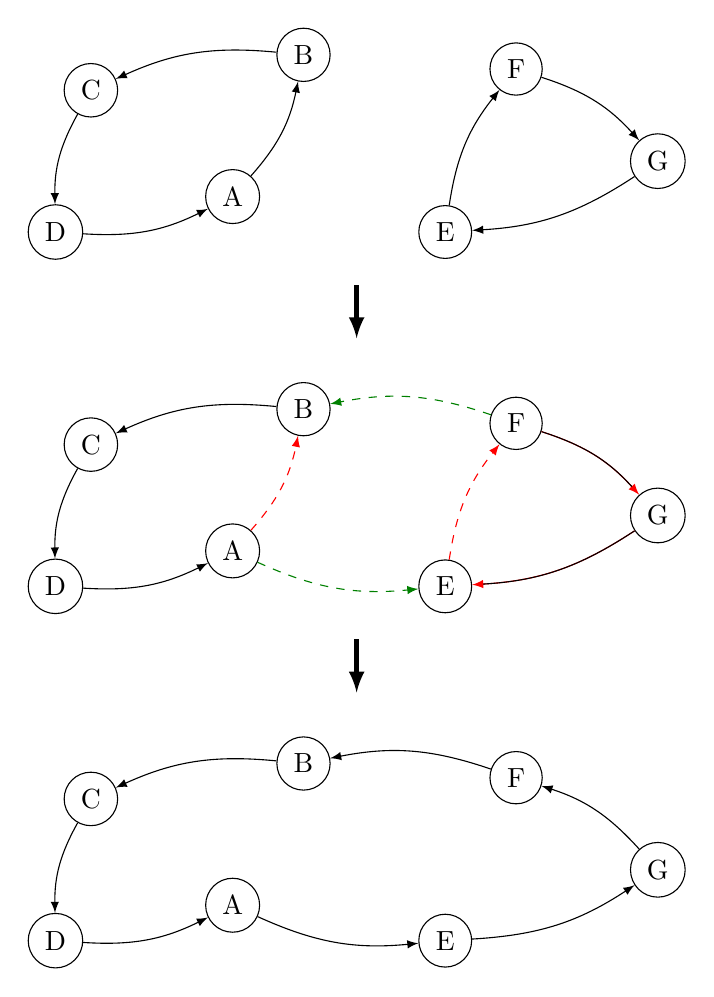
\begin{tikzpicture}[scale=0.9]

			\begin{scope}[shift={(0, 0)}]
	            \node[circle, draw, fill=white] (A) at (0,0) {A};
	            \node[circle, draw, fill=white] (B) at (1,2) {B};
	            \node[circle, draw, fill=white] (C) at (-2,1.5) {C};
	            \node[circle, draw, fill=white] (D) at (-2.5,-0.5) {D};
	            \node[circle, draw, fill=white] (E) at (3,-0.5) {E};
	            \node[circle, draw, fill=white] (F) at (4,1.8) {F};
	            \node[circle, draw, fill=white] (G) at (6,0.5) {G};
	        
	            \draw[-latex] (A) to[bend right=15] (B);
	            \draw[-latex] (B) to[bend right=15] (C);
	            \draw[-latex] (C) to[bend right=15] (D);
	            \draw[-latex] (D) to[bend right=15] (A);
	            \draw[-latex] (E) to[bend left=15] (F);
	            \draw[-latex] (F) to[bend left=15] (G);
	            \draw[-latex] (G) to[bend left=15] (E);

				\draw[-latex,ultra thick] (1.75,-1.25) -- (1.75,-2);
	        \end{scope}

			\begin{scope}[shift={(0, -5)}]
	            \node[circle, draw, fill=white] (A) at (0,0) {A};
	            \node[circle, draw, fill=white] (B) at (1,2) {B};
	            \node[circle, draw, fill=white] (C) at (-2,1.5) {C};
	            \node[circle, draw, fill=white] (D) at (-2.5,-0.5) {D};
	            \node[circle, draw, fill=white] (E) at (3,-0.5) {E};
	            \node[circle, draw, fill=white] (F) at (4,1.8) {F};
	            \node[circle, draw, fill=white] (G) at (6,0.5) {G};
	        
	            \draw[-latex,dashed,Red] (A) to[bend right=15] (B);
	            \draw[-latex,dashed,Green] (A) to[bend right=15] (E);
	            \draw[-latex] (B) to[bend right=15] (C);
	            \draw[-latex] (C) to[bend right=15] (D);
	            \draw[-latex] (D) to[bend right=15] (A);
	            \draw[-latex,dashed,Red] (E) to[bend left=15] (F);
	            \draw[-latex,dashed,Green] (F) to[bend right=15] (B);
	            \draw[-latex,Red] (F) to[bend left=15] (G);
	            \draw[-latex,Red] (G) to[bend left=15] (E);
	            \draw[-,shorten >=4pt,] (F) to[bend left=15] (G);
	            \draw[-,shorten >=4pt,] (G) to[bend left=15] (E);

				\draw[-latex,ultra thick] (1.75,-1.25) -- (1.75,-2);
	        \end{scope}

			\begin{scope}[shift={(0, -10)}]
	            \node[circle, draw, fill=white] (A) at (0,0) {A};
	            \node[circle, draw, fill=white] (B) at (1,2) {B};
	            \node[circle, draw, fill=white] (C) at (-2,1.5) {C};
	            \node[circle, draw, fill=white] (D) at (-2.5,-0.5) {D};
	            \node[circle, draw, fill=white] (E) at (3,-0.5) {E};
	            \node[circle, draw, fill=white] (F) at (4,1.8) {F};
	            \node[circle, draw, fill=white] (G) at (6,0.5) {G};
	        
	            \draw[-latex] (A) to[bend right=15] (E);
	            \draw[-latex] (B) to[bend right=15] (C);
	            \draw[-latex] (C) to[bend right=15] (D);
	            \draw[-latex] (D) to[bend right=15] (A);
	            \draw[-latex] (F) to[bend right=15] (B);
	            \draw[-latex] (G) to[bend right=15] (F);
	            \draw[-latex] (E) to[bend right=15] (G);

	        \end{scope}
		\end{tikzpicture}
	\end{center}
	\caption{Example of merging two subtours} \label{fig:examplePatching}
\end{figure}

\begin{figure}[htbp]
	\textbf{Patching Heuristic} \\
	\begin{algorithm}[H]
		\SetKwInOut{Input}{input}
		\SetKwInOut{Output}{output}
		\Input{
			Graph $G(V,E)$ fully connected \newline
			$c_{ij}=$ cost of $edge(i,j) \in |E|$ $\forall$ $i,j \in V$ with $i \neq j$ \newline
			$S$ solution containing two or more subtours
			}
		\Output{Valid solution $S$}
		\vspace{2mm}
		$count \gets$ number of subtours in $S$ \\
		\While{$count > 1$ }{
			$e_{i,j} \in s_1$, $e_{k,l} \in s_2$ $\gets$ Find Best Patching Edges \\%(procedure similar to 2opt) \\
			merge $s_1$ with $s_2$ by swapping $e_{i,j}$, $e_{k,l}$ with $e_{i,l}$, $e_{k,j}$ (or with $e_{i,k}$, $e_{j,l}$ if it is cheaper on the cost) \\
			$count \gets count - 1$ 
		}
		\Return{$S$}
	\end{algorithm}
	\caption{Patching Heuristic pseudocode} \label{fig:patchHeur}
\end{figure}

With this method the chance of Benders of not producing any solution is greatly reduced, but not nullified since CPLEX needs to finish at least once.
Patching Heuristic allows to generate a new solution at each iteration of Benders and, as the number of SEC added increases the quality of such solution usually increases.
This happens because the solution that is produced resembles more and more an optimal solution as Benders iterates, sometimes it even happens that an optimal solution is found by patching subtours before the end of Benders, however the only way to verify optimality is to wait for the algorithm to finish.
Furthermore this technique can be applied together with warm starting: by keeping the best solution obtained, at each iteration such solution can be used to warm start cplex.
Since better solutions than the first warm starting solution are likely to be produced at some point, efficiency of subtree pruning will also increase as the best solution quality improves, resulting, theoretically, in better efficiency.

\subsection{Efficiency}
Benders, being an exact algorithm, automatically stops once it finds the optimal solution and the runtime changes at every run in a random way, depending on the random seed of CPLEX. 
This means that it's more interesting to study time efficiency than the performance given by the cost of the resulting solution.
Since the algorithm is quite slow the instances on which it has run are all below 1000 nodes\footnote{Instances ts225 and p654 were excluded since for some reason the solving time on those is way higher compared to the others. Such difference would offset too much time limits hence they were removed}, with an increased time limit compared to previous testing which allowed to always reach optimality.
Specifying the time limit is mandatory since some of the tests use warm start which requires a global time limit to obtain it's own time limit that is set to either 5\% or 1\%.
% \tablename{ \ref{tab:bendersSimple}} contains the average runtime of Benders of five runs on each instance with different seeds, however it must be noted that time used to find the warm starting solution is not included.
The time limits used to gather data as set according to \tablename{ \ref{tab:bendersTlims}}.

\begin{table}[htbp]
	\centering
	\caption{Time limits used to run benders while gathering data} \label{tab:bendersTlims}	\vspace{2mm}
	\begin{tabular}{|C{22mm}|C{21mm}|C{28mm}|C{28mm}|}
		\hline \multirow{2}{22mm}{\textbf{Nodes range}} & \multicolumn{3}{c|}{\textbf{Time Limits}} \\ 
		\cline{2-4} & \textbf{Global} & \textbf{Warm Start 5\%} & \textbf{Warm Start 1\%} \\
		\hline
		0 - 80 & 5 seconds & 0.25 seconds & 0.05 seconds\\
		100 - 200 & 30 seconds & 1.5 seconds & 0.3 seconds\\
		220 - 320 & 120 seconds & 6 seconds & 1.2 seconds\\
		400 - 500 & 300 seconds & 15 seconds & 3 seconds\\
		500 - 800 & 400 seconds & 20 seconds & 4 seconds\\
		\hline
	\end{tabular}
\end{table} 
 
% \vspace{5mm}
% \begin{longtable}{L{15mm}C{15mm}C{22mm}C{18mm}C{22mm}}
% 	\caption{Benders only runtimes in seconds (with 1\% time limit on warm start)} \label{tab:bendersSimple}\\
% 	\endfirsthead
% 	\textbf{Instance} & \textbf{Basic} & \textbf{Warm Start} & \textbf{Patching} & \textbf{Warm Start + Patching}
% 	\endhead
% 	\textbf{Instance} & \textbf{Basic} & \textbf{Warm Start} & \textbf{Patching} & \textbf{Warm Start + Patching}
% 	\csvreader[head to column names]{csv/benders_simple-runtime.csv}{}% use head of csv as column names
% 	{\\ \csvcoli & \csvcolii & \csvcoliii & \csvcoliv & \csvcolv}% specify your coloumns here
% 	\\
% \end{longtable}

\begin{figure}[htbp]
	\centering 
	\begin{tikzpicture}
        \begin{axis}[
            xlabel={Time Ratio},     % AXIS NAME
            %ylabel={Iterations/s Ratio},   % AXIS NAME
            xmin=1, xmax=1.8,       % AXIS LIMITS
            ymin=0, ymax=47,        % AXIS LIMITS
            xtick={},
            ytick=\empty,
            legend style={at={(0.98,0.02)},anchor=south east,legend columns=1}, %MOVE LEGEND HERE
			legend cell align={left},
            %ymajorgrids=true,
            xmajorgrids=true,
            grid style=dashed,
        ]
        
        \addplot[Blue,mark=square,mark size=1.5] table[x=simple_base,y=idx, col sep=semicolon] {csv/benders_runtimes.csv}; 
        \addplot[Red,mark=o,mark size=1.5] table[x=simple_ws1,y=idx, col sep=semicolon] {csv/benders_runtimes.csv};
        \addplot[Green,mark=triangle,mark size=1.5] table[x=simple_ws5,y=idx, col sep=semicolon] {csv/benders_runtimes.csv}; 
        \addplot[Purple,mark=star,mark size=1.5] table[x=simple_patch,y=idx, col sep=semicolon] {csv/benders_runtimes.csv}; 
        \addplot[Dandelion,mark=otimes,mark size=1.5] table[x=simple_patch+ws1,y=idx, col sep=semicolon] {csv/benders_runtimes.csv}; 
        \addplot[Black,mark=diamond,mark size=1.5] table[x=simple_patch+ws5,y=idx, col sep=semicolon] {csv/benders_runtimes.csv}; 
        \addlegendentry{Basic} 
        \addlegendentry{Warm start 1\%}
        \addlegendentry{Warm start 5\%}
        \addlegendentry{Patching}
        \addlegendentry{Patching + Warm start 1\%}
        \addlegendentry{Patching + Warm start 5\%}
            
        \end{axis}
    \end{tikzpicture}
	\caption{Performance profile graph on runtimes of benders \label{fig:bendersSimplePerfProf}}
\end{figure}

To obtain a more insightful comparison \figurename{ \ref{fig:bendersSimplePerfProf}} compares all average runtimes collected exluding warm start time.
The basic version of Benders falls short of the ones that use patching and warm start basically every time, while it's clear that using any kind of warm starting, including its combination with Patching, improves efficiency by a noticeable amount.
Starting Benders usign an already existing solution seems to also have an improving effect, with the better solution, that is intuitevly found by spending more time on its computation, yielding an improvement very small that could very well be considered within standard deviation of tests when Patching is applied as well.
However the time taken to find that first solution must also be taken into account.

\begin{figure}[htbp]
	\centering
	\begin{tikzpicture}
        \begin{axis}[
            xlabel={Time Ratio},     % AXIS NAME
            %ylabel={Iterations/s Ratio},   % AXIS NAME
            xmin=1, xmax=3,       % AXIS LIMITS
            ymin=0, ymax=47,        % AXIS LIMITS
            xtick={},
            ytick=\empty,
            legend style={at={(0.98,0.02)},anchor=south east,legend columns=1}, %MOVE LEGEND HERE
			legend cell align={left},
            %ymajorgrids=true,
            xmajorgrids=true,
            grid style=dashed,
        ]
        
        \addplot[Blue,mark=square,mark size=1.5] table[x=full_base, y=idx, col sep=semicolon] {csv/benders_runtimes.csv}; 
        \addplot[Red,mark=o,mark size=1.5] table[x=full_ws1, y=idx, col sep=semicolon] {csv/benders_runtimes.csv};
        \addplot[Green,mark=triangle,mark size=1.5] table[x=full_ws5, y=idx, col sep=semicolon] {csv/benders_runtimes.csv}; 
        \addplot[Purple,mark=star,mark size=1.5] table[x=full_patch, y=idx, col sep=semicolon] {csv/benders_runtimes.csv}; 
        \addplot[Dandelion,mark=otimes,mark size=1.5] table[x=full_patch+ws1, y=idx, col sep=semicolon] {csv/benders_runtimes.csv}; 
        \addplot[Black,mark=diamond,mark size=1.5] table[x=full_patch+ws5, y=idx, col sep=semicolon] {csv/benders_runtimes.csv}; 
        \addlegendentry{Basic} 
        \addlegendentry{Warm start 1\%}
        \addlegendentry{Warm start 5\%}
        \addlegendentry{Patching}
        \addlegendentry{Patching + Warm start 1\%}
        \addlegendentry{Patching + Warm start 5\%}
            
        \end{axis}
    \end{tikzpicture}
	\caption{Performance profile graph on runtimes of benders including warm start time \label{fig:bendersFullPerfProf}}
\end{figure}

In \figurename{ \ref{fig:bendersFullPerfProf}} it's clear to see that the time needed to get the first solution using external means than Benders is actually greatly affecting the efficiency of the run in a negative way.
The efficiency decreases so much that even the basic version of Benders is on par or better, while the best for overall runtime is given by only Patching.
It's also possible to advance the hypothesis that the first solution doesn't need to be a strictly good one when Patching is involved, since Patching will find a better solutions during the execution, it would be beneficial to define a specific way to find the first solution in order to waste least possible amount of time on it.
Further testing may be considered to be done on top of such hypothesis by using even less time to find the first warm starting solution, that however is outside of the scope of this project.

% \newpage

\section{Branch and Cut}
Branch and Cut is a method that builds upon the Branch and Bound technique and improves it using knowledge specific on the problem domain to find more efficient cuts.
The simplest way to implement this algorithm is to check for subtours and add necessary SEC directly within \textit{CPXmipopt}.
To achieve this CPLEX allows the user to define some code that will be called while CPLEX solver itself is running, thus allowing to add SEC before \textit{CPXmipopt} terminates losing the cut pool and other useful informations.
The generic callback technique allows to run user codes at specified points in the execution, like when a candidate solution is found or when the LP relaxation is solved.
For the most simple implementation of Branch and Cut the callback code is just needed to run upon discovering a solution candidate so such solution can be checked for subtours and SEC can be added to the cut pool.

\begin{figure}[htbp]
	\textbf{Basic Candidate Callback} \\
	\begin{algorithm}[H]
		\SetKwInOut{Input}{input}
		\Input{ 
			CPLEX problem $p$ \newline
			candidate solution $x$ \newline
			best solution found until now $b$
		}
		\vspace{2mm}
		$t \gets$ convert $x$ to successors solution\\
		\uIf{number of subtours in $t$ $>$ 1}{
			\ForEach{subtour $s \in t$}{ 
				add SEC violated by $s$ to $p$ \\
			}
			reject candidate $x$ \\
		}
		\uElseIf{cost($t$) $<$ cost($b$) }{$b \gets t$}
	\end{algorithm}
	\caption{Basic Callback function} \label{fig:callbackBase}
\end{figure}
\begin{figure}[htbp]
	\textbf{Branch and Cut} \\
	\begin{algorithm}[H]
		\SetKwInOut{Input}{input}
		\SetKwInOut{Output}{output}
		\Input{Graph $G(V,E)$ fully connected }
		\Output{Optimal Solution $x^*$}
		\vspace{2mm}
		$p \gets$ CPLEX Initialization (\ref{fig:CPLEXinit})\\
		set CPLEX callback function \textbf{Candidate Callback}\\
		$x^* \gets$ optimal solution of $p$\\
		\Return{$x^*$}
	\end{algorithm}
	\caption{Branch and Cut algorithm} \label{fig:branchAndCut}
\end{figure}

The Branch and Cut algorithm implemented this way still has the same weakness of Benders: it's not sure that a feasible solution will be produced until the optimal solution is found.
The problem is solved the same way as Benders's, it's simply necessary to run Patching Heuristic and every time a candidate is found a feasible solution will be produced as well.
With the same reasoning the warm start procedure can also be applied.

\subsection{Posting}
During the execution of Branch and Cut it's possible for a solution better than the ones observed before it to apper while navigating the search tree.
Solutions obtained this way cannot be used to warm start CPLEX because in this Branch and Cut implementation there is only one chance for a warm start, that is at the very beginning since \textit{CPXmipopt} runs only once.
To allow CPLEX to reap similar benefits of the warm start and Patching of Benders while the solver is running a similar but callback-specific operation called Posting needs to be performed.
The Posting procedure allows the user to give CPLEX a feasible solution during the solving procedure to improve the pruning of the search tree yielding overall better time efficiency.
A feasible solution to use in the Posting procedure can be either found as candidate while exploring the search tree or by patching an invalid candidate solution.
Posting can be viewed as a low level implementation of the warm start technique as the advantages given by both methods are indeed very similar.
With the implementation of the solution posting the candidate callback is complete and it's shown in \figurename{ \ref{fig:callbackComplete}}

\begin{figure}[htbp]
	\textbf{Complete Candidate Callback} \\
	\begin{algorithm}[H]
		\SetKwInOut{Input}{input}
		\Input{ 
			CPLEX problem $p$ \newline
			candidate solution $x$ \newline
			best solution found until now $b$
		}
		\vspace{2mm}
		$t \gets$ convert $x$ to successors solution\\
		\uIf{number of subtours in $t$ $>$ 1}{
			\ForEach{subtour $s \in t$}{ 
				add SEC violated by $s$ to $p$ \\
			}
			reject candidate $x$ \\
			$t \gets$ \textbf{Patching Heuristic}($t$) (\ref{fig:patchHeur})
		}
		\tcc{$t$ is certainly a valid solution at point}
		\uIf{cost($t$) $<$ cost($b$) }{
			$b \gets t$\\
			\textbf{Post Solution} $t$
		}
	\end{algorithm}
	\caption{Candidate callback implementing both patching and posting} \label{fig:callbackComplete}
\end{figure}

\subsection{Concorde and  Usercuts}

The Concorde TSP Solver, developed by William Cook and his collaborators, is one of the most advanced and effective tools for solving large-scale instances of the TSP.
Using it as a C library, Concorde provides with multiple useful functions including those that allow to compute advanced cuts on a fractional solution in Branch and Cut.
These cuts come in the form simple Gomory cuts as well as TSP specific cuts, which allow to add SEC in advance, avoiding spending time to reach some invalid candidate solutions, although not avoiding them entirely.
A brief description on how these specific cuts are found is described below.
Initially, the LP relaxation of the TSP is solved, where the integer constraints on the decision variables \( x_{ij} \) are relaxed, allowing them to take fractional values between 0 and 1.
The resultant solution provides fractional edge values \( x_{ij}^* \), representing the degree to which each edge \( (i,j) \) is included in the tour.
Using the fractional solution, a residual graph \( G = (V, E) \) is constructed.
In this graph, nodes \( V \) correspond to cities, and edges \( E \) are weighted by the fractional values \( x_{ij}^* \), which serve as the capacities of the edges.
To identify violated subtour elimination constraints, a maximum flow algorithm is employed.
By selecting a source node \( s \) and a sink node \( t \) from the graph, the maximum flow from \( s \) to \( t \) is computed.
The maximum flow value corresponds to the minimum capacity cut that separates \( s \) from \( t \).
The min cut found after computing the max flow separates the graph into two disjoint subsets \( S \) and \( T \).
The sum of the capacities of the edges crossing from \( S \) to \( T \) is minimized.
If the sum of the fractional values \( x_{ij}^* \) across the cut is less than \( |S| - 1 \), it indicates that this cut violates the subtour elimination constraint, implying the existence of a subtour that does not connect all nodes in a single tour.
Upon identifying a violated subtour elimination constraint, it is added to the LP formulation and the procedure then continues.

In order for the procedure above to work it needs to get as input the solution at the LP relaxation point, thus requiring to complicate a bit the callback function.
In fact before it was said that the callback was only executed on discovering a new candidate solution which is an integer solution.
To obtain access to the relaxation solution it is necessary to let CPLEX invoke the callback at both candidate and relaxation point, dividing the callback into two parts.
That said the candidate callback remains the same while the relaxation callback, \figurename{ \ref{fig:relaxCallback}}, is the one which implements usercuts.

\begin{figure}[htbp]
	\textbf{Relaxation Callback} \\
	\begin{algorithm}[H]
		\SetKwInOut{Input}{input}
		\Input{ 
			CPLEX problem $p$ \newline
			relaxation optimal solution $x$ \newline
		}
		\vspace{2mm}
		$comps \gets$ \textbf{CCcut\_connect\_components}($x$) \\
		\uIf{number of components in $comps$ $>$ 1}{
			\tcp{If multiple components are detected add cuts to invalidate them}
			\ForEach{component $c \in comps$}{ 
				add SEC violated by $c$ to $p$ as usercut\\
			}
		}
		\uElseIf{number of components in $comps$ $=$ 1}{
			\tcp{If only one component is detected use Concorde to find the best cut/cuts}
			$cuts \gets$ \textbf{CCcut\_violated\_cuts}($x$)\\
			\ForEach{cut $c \in cuts$}{ 
				add cut by $c$ to $p$ as usercut\\
			}
		}
	\end{algorithm}
	\caption{Relaxation Callback implementing usercuts using Concorde library} \label{fig:relaxCallback}
\end{figure}

\subsection{Efficiency}
For the same reason explained with Benders, this section will discuss the effectiveness of each of the strategies described above using the execution time as the main metric.
\begin{figure}[htbp]
	\centering
	\begin{tikzpicture}
        \begin{axis}[
            xlabel={Time Ratio},     % AXIS NAME
            %ylabel={Iterations/s Ratio},   % AXIS NAME
            xmin=1, xmax=3,       % AXIS LIMITS
            ymin=0, ymax=47,        % AXIS LIMITS
            xtick={},
            ytick=\empty,
            legend style={at={(0.98,0.02)},anchor=south east,legend columns=1,cells={align=left}}, %MOVE LEGEND HERE
			legend cell align={left},
            %ymajorgrids=true,
            xmajorgrids=true,
            grid style=dashed,
        ]
        
        \addplot[Blue,mark=square,mark size=1.5] table[x=full_base, y=idx, col sep=semicolon] {csv/branch-cut_runtimes.csv}; 
        \addplot[Red,mark=o,mark size=1.5] table[x=full_post, y=idx, col sep=semicolon] {csv/branch-cut_runtimes.csv};
        \addplot[Green,mark=triangle,mark size=1.5] table[x=full_usercut, y=idx, col sep=semicolon] {csv/branch-cut_runtimes.csv}; 
        \addplot[Purple,mark=star,mark size=1.5] table[x=full_post+usercut, y=idx, col sep=semicolon] {csv/branch-cut_runtimes.csv}; 
        \addplot[Dandelion,mark=otimes,mark size=1.5] table[x=full_post+usercut+ws1, y=idx, col sep=semicolon] {csv/branch-cut_runtimes.csv};
        \addlegendentry{Basic} 
        \addlegendentry{Posting}
        \addlegendentry{Usercuts}
        \addlegendentry{Posting + Usercuts}
        \addlegendentry{Posting + Usercuts\\ + Warm start 1\%}
            
        \end{axis}
    \end{tikzpicture}
	\caption{Performance profile graph on the execution time of the whole program using Branch and Cut algorithm \label{fig:branchCutFull}}
\end{figure}
By inspecting \figurename{ \ref{fig:branchCutFull}} it's possible to see that the best possible configuration of the Branch and Cut method is a cobination of both Posting and Usercuts, with what it seems to be a more impactful improvement given by the latter.
Posting alone is still able to outperform the basic version of the algorithm, while using warm start is not the worst combination, managing to perform slightly worse than Posting.
The tables turn completely when not taking into consideration the warm start time.
\begin{figure}[htbp]
	\centering
	\begin{tikzpicture}
        \begin{axis}[
            xlabel={Time Ratio},     % AXIS NAME
            %ylabel={Iterations/s Ratio},   % AXIS NAME
            xmin=1, xmax=3,       % AXIS LIMITS
            ymin=0, ymax=47,        % AXIS LIMITS
            xtick={},
            ytick=\empty,
            legend style={at={(0.98,0.02)},anchor=south east,legend columns=1,cells={align=left}}, %MOVE LEGEND HERE
			legend cell align={left},
            %ymajorgrids=true,
            xmajorgrids=true,
            grid style=dashed,
        ]
        
        \addplot[Blue,mark=square,mark size=1.5] table[x=simple_base, y=idx, col sep=semicolon] {csv/branch-cut_runtimes.csv}; 
        \addplot[Red,mark=o,mark size=1.5] table[x=simple_post, y=idx, col sep=semicolon] {csv/branch-cut_runtimes.csv};
        \addplot[Green,mark=triangle,mark size=1.5] table[x=simple_usercut, y=idx, col sep=semicolon] {csv/branch-cut_runtimes.csv}; 
        \addplot[Purple,mark=star,mark size=1.5] table[x=simple_post+usercut, y=idx, col sep=semicolon] {csv/branch-cut_runtimes.csv}; 
        \addplot[Dandelion,mark=otimes,mark size=1.5] table[x=simple_post+usercut+ws1,y=idx, col sep=semicolon] {csv/branch-cut_runtimes.csv};
        \addlegendentry{Basic} 
        \addlegendentry{Posting}
        \addlegendentry{Usercuts}
        \addlegendentry{Posting + Usercuts}
        \addlegendentry{Posting + Usercuts\\ + Warm start 1\%}
            
        \end{axis}
    \end{tikzpicture}
	\caption{Performance profile graph on the execution time of the Branch and Cut algorithm (excluding warm start time) \label{fig:branchCutSimple}}
\end{figure}
As \figurename{ \ref{fig:branchCutSimple}} clearly shows, the time took by Branch and Cut to solve an instance using the warm start technique in combination with both Posting and Usercuts, is undoubtely the best.
Such a result is very similar to Benders's case of warm starting, where the efficiency using warm start would be hindered by the first solution time.
This situation gives more gravity to a matter secondary to the algorithm itself: what is the exact time needed obtain a good enough solution to use as warm start while not deteriorating the algorithm efficiency as a whole?
An interesting experiment would be to run again all tests while instead of optimizing the warm start solution according to a time limit, obtain the first possible solution and optimizing it according to a number of iterations.
As an example the first solution could be obtained by running Nearest Neightbor $k$ times with $k=10$ or some other reasonably low value and than optimize the best solution obtained using 2-Opt.
Since such kind of experiment would require major changes to the project code it was deemed outside the scope of the project. 

\section{Comparison}	
Finally \figurename{ \ref{fig:bendersBranchCut}} directly compares Benders method and Branch and Cut algorithm, both with and without using the warm starting technique.
On average Branch and Cut runs three times faster compared to Benders, however, in some instances, the latter still outperforms the first.

\begin{figure}[htbp]
	\centering
	\begin{tikzpicture}
        \begin{axis}[
            xlabel={Time Ratio},     % AXIS NAME
            %ylabel={Iterations/s Ratio},   % AXIS NAME
            xmin=1, xmax=10,       % AXIS LIMITS
            ymin=0, ymax=47,        % AXIS LIMITS
            xtick={},
            ytick=\empty,
            legend style={at={(0.98,0.02)},anchor=south east,legend columns=1,cells={align=left}}, %MOVE LEGEND HERE
			legend cell align={left},
            %ymajorgrids=true,
            xmajorgrids=true,
            grid style=dashed,
        ]
        
        \addplot[Blue,mark=square,mark size=1.5] table[x=ben, y=idx, col sep=semicolon] {csv/cmp_benders-branch-cut_full.csv}; 
        \addplot[Red,mark=o,mark size=1.5] table[x=bran, y=idx, col sep=semicolon] {csv/cmp_benders-branch-cut_full.csv};
        \addplot[Green,mark=triangle,mark size=1.5] table[x=ben+ws1, y=idx, col sep=semicolon] {csv/cmp_benders-branch-cut_full.csv}; 
        \addplot[Purple,mark=star,mark size=1.5] table[x=bran+ws1, y=idx, col sep=semicolon] {csv/cmp_benders-branch-cut_full.csv};
        \addlegendentry{Benders} 
        \addlegendentry{Branch \& Cut}
        \addlegendentry{Benders + Warm start 1\%}
        \addlegendentry{Branch \& Cut + Warm start 1\%}
            
        \end{axis}
    \end{tikzpicture}
	\caption{Comparison between Benders and Branch and Cut\label{fig:bendersBranchCut}}
\end{figure}